\chapter{StageBridge: Materials and Methods} \label{chap:methods}

%% Chapter 3 = the StageBridge model (single model; CRRT-UDE is a descriptive technical label, not a
%% second branded method). VOICE: declarative, bold; no negate-first; honesty in the limitations.
%% Equations numbered; every variable defined (Systems-Bio convention). Methods subsections = noun phrases.
%% Names: StageBridge (the model); Merchavit (Rust BANKSY); SDRA; Hierarchical Set Transformer.
%% Corrections reflected: low-rank identifiable A = U V (rank 32); source-fixed context w(tau)=w_i primary.

\section{Overview}

Chapter~\ref{chap:intro} argued that premalignant progression is a tissue-level process and posed
three pre-specified hypotheses about whether, through which regulatory programs, and at what spatial
scale local tissue context alters epithelial progression. This chapter builds the method that
operationalizes and tests them. Its design is disciplined by adversarial validation: the transport
coupling that defines the estimand was selected against a frozen synthetic benchmark with known ground
truth, and an initial formulation that failed that benchmark was discarded before any real data were
analyzed (Section~\ref{sec:selection}).

StageBridge is a context-residual universal differential equation framework for learning
progression-associated regulatory transport from cross-sectional spatial omics. It models premalignant
epithelial progression as a receiver-centered transition problem: each focal epithelial unit is a
\emph{receiver} whose progression-aligned behavior is modeled, and its surrounding tissue is the
\emph{local context} that may redirect that behavior. StageBridge is built to separate three
contributions to a receiver's progression that a static tissue snapshot ordinarily confounds:
receiver-intrinsic progression, specimen-level ecology, and genuinely local niche redirection. The
central object of inference is the \emph{context residual} $R_{\mathrm{cond}}$: the component of the
epithelial transition field that local cell-state context explains after the receiver's own state and
the ordered stage edge are accounted for.

The implementation evaluated in this thesis uses fixed regulatory receiver states, precomputed
spatial-context features, conditional-stratified optimal transport, and conditional flow matching. This
chapter defines the progression-inference problem (Section~\ref{sec:problem}), the design principles
that organize the model (Section~\ref{sec:principles}), the unified dynamical formulation
(Section~\ref{sec:field}), the receiver and context representations
(Sections~\ref{sec:receiver-rep}--\ref{sec:context-rep}), the transport coupling
(Section~\ref{sec:coupling}), the context-residual estimand (Section~\ref{sec:estimand}), the training
procedure (Section~\ref{sec:training}), and the identifiability screen and falsification ladder
(Section~\ref{sec:selection}--\ref{sec:ladder}). Section~\ref{sec:config} states exactly what produced
the results of the following chapter and names the architectural extension that completes the model.
Figure~\ref{fig:core-schematic} summarizes the evaluated implementation.

\begin{figure}[htbp]
\centering
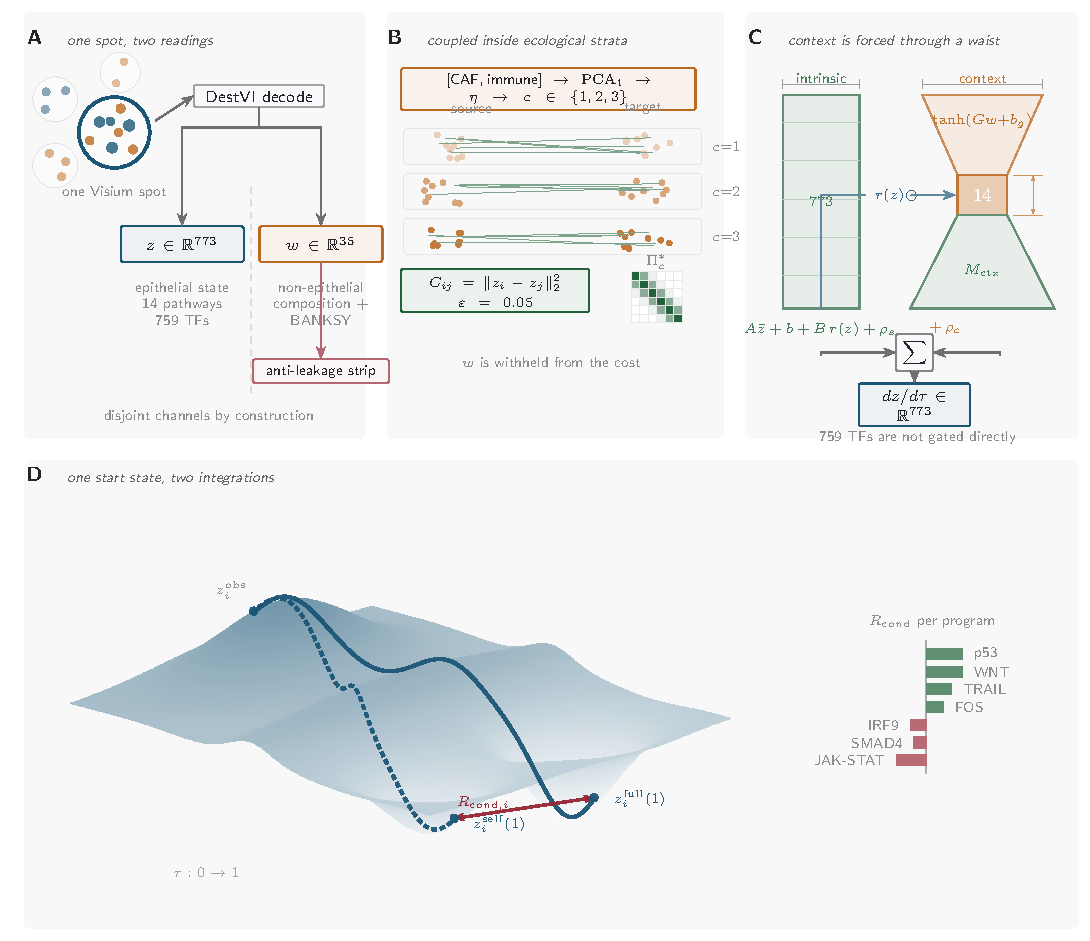
\includegraphics[width=\textwidth]{crrt_ude_schematic.pdf}
\caption{StageBridge schematic (evaluated implementation). Each epithelial receiver carries a
regulatory state $z$ (PROGENy pathways and CollecTRI transcription factors) and a spatial context
vector $w$ (deconvolution-derived composition and Merchavit spatial features). The vector field
decomposes into a receiver-intrinsic self term $v_{\mathrm{self}}$ and a tanh-gated context term
$v_{\mathrm{context}}$; integrating from a common initial state in self versus full mode yields the
per-receiver context residual $R_{\mathrm{cond}}$.}
\label{fig:core-schematic}
\end{figure}

\section{Data and preprocessing}
\label{sec:data}

\subsection{Cohorts}

The LUAD cohort draws on the publicly available lung adenocarcinoma progression atlas, spanning
five morphological stages: Normal, atypical adenomatous hyperplasia (AAH), adenocarcinoma in situ
(AIS), minimally invasive adenocarcinoma (MIA), and invasive LUAD. The atlas provides paired
single-nucleus RNA-seq and Visium spatial transcriptomics. The transport \emph{receivers} are the
Visium spots: each spot's epithelial regulatory state $z$ is read from its DestVI-decoded epithelial
expression and its context $w$ from the surrounding non-epithelial ecology (below), so a receiver is a
spatial spot, not a dissociated single nucleus. The single-nucleus data serve as the deconvolution and
cell-type reference and for the co-expression analyses, not as transport receivers. Donors were assigned to patient-held-out cross-validation folds
(Section~\ref{sec:estimand}) prior to any analysis; no patient contributes to both
training and evaluation on any edge. The PanIN cohort consists of graded pancreatic
intraepithelial neoplasia Visium spatial transcriptomics sections, processed through the same
pipeline with a low-grade vs high-grade edge.

\subsection{Regulatory program scoring}

Regulatory activities were computed on log-normalized expression using decoupleR \autocite{Badia-I-Mompel2022-te}.
PROGENy pathway activities (14 pathways) and CollecTRI transcription-factor activities
(759 TFs) were estimated by univariate linear model (ULM) to produce a cells$\times$773
regulatory-program matrix $z$. This matrix is the receiver state space in which all
transport, matching, and interpretation are defined.

\subsection{Spatial context features}

Spatial neighborhood features were computed with Merchavit, a Rust implementation of the BANKSY
spatial-context algorithm \autocite{Singhal2024-rv}, applied independently within each tissue
section. BANKSY augments each cell's own expression with a weighted mean and a weighted
gradient of its spatial neighbors' expression, capturing the composition and structure of the
immediate tissue environment. Cell-type composition per spot was estimated by DestVI
deconvolution \autocite{Lopez2022-ps} against the Lung Cancer Atlas single-cell
reference \autocite{Salcher2022-pu}. The assembled context vector $w$ contains broad non-epithelial
composition fractions (cancer-associated fibroblast, immune, myeloid, stromal, lymphoid, and
endothelial), spatial BANKSY features, and the regulatory program scores of the surrounding
\emph{non-epithelial} cells; the receiver's own epithelial regulatory state is excluded from $w$
by construction (Section~\ref{sec:context-rep}), so context and receiver state are disjoint.

\section{The progression-inference problem}\label{sec:problem}

Let a receiver be indexed by $i$. Each receiver carries a regulatory state
$z_i \in \mathbb{R}^{d_z}$, a spatial context vector $w_i \in \mathbb{R}^{d_w}$, and a discrete stage
label from an ordered progression. For lung adenocarcinoma the sequence is
$\mathrm{Normal} \to \mathrm{AAH} \to \mathrm{AIS} \to \mathrm{MIA} \to \mathrm{invasive\ LUAD}$; for
pancreatic intraepithelial neoplasia it is low-grade to high-grade PanIN. Progression along a single
ordered edge is parameterized by a normalized pseudo-time $\tau \in [0,1]$, where $\tau=0$ denotes the
source stage and $\tau=1$ the target stage. The state $z_i$ is an epithelial-intrinsic quantity
(Section~\ref{sec:receiver-rep}); the context $w_i$ summarizes the non-epithelial tissue ecology
surrounding receiver $i$ (Section~\ref{sec:context-rep}).

The data are cross-sectional: no receiver is observed at both $\tau=0$ and $\tau=1$, and there is no
observed longitudinal correspondence between a source cell and the target cell it becomes. The modeling
question is stated in two forms. Informally: given a receiver's epithelial state and an ordered stage
edge, which local cell-state contexts are associated with residual changes in the inferred transition
behavior? Formally: for a learned transition field $v(z, w, \tau)$, does the context-dependent
component of $v$ carry information about the progression endpoint beyond the receiver-intrinsic
component, after holding the receiver state $z$ and the stage edge fixed? The context residual
$R_{\mathrm{cond}}$ of Section~\ref{sec:estimand} makes this comparison the direct object of inference
rather than an annotation applied after transition modeling.

\section{StageBridge design principles}\label{sec:principles}

StageBridge is organized by three principles. The first is a \emph{receiver-centered} view of
transition: information flows to a receiver from its neighborhood, and the model asks what a cell
receives from its surroundings. This mirrors the framing that a therapy is administered to a patient
rather than to a tumor in isolation, so that the environment a cell inhabits, and not only its own
genome, shapes its trajectory. The second is that matching, transport, and interpretation are carried
out in a \emph{semantic} feature space whose coordinates are named biological programs, so a context
effect reads directly as an effect on a specific pathway or regulator rather than on an opaque latent
dimension. The third is that the transition field is \emph{structured}: it is written as interpretable
algebraic terms combined with small learned residuals, following a universal differential equation
(UDE) parameterization, so the learned dynamics remain readable.

These principles motivate a target separation of three contributions to a receiver's progression:
\begin{equation}\label{eq:separation}
\underbrace{\text{receiver-intrinsic progression}}_{\text{cell's own state}}
\quad\text{vs.}\quad
\underbrace{\text{specimen ecology}}_{\text{donor/stage-level environment}}
\quad\text{vs.}\quad
\underbrace{\text{local niche redirection}}_{\text{cell's own microenvironment}} .
\end{equation}
The evaluated implementation separates receiver-intrinsic progression from context
(Section~\ref{sec:field}), and the falsification ladder of Section~\ref{sec:ladder} separates
specimen-level ecology from genuinely local niche effects empirically by comparing a donor/stage-average
context against each receiver's own local context. An explicit architectural decomposition of the
context into a specimen-average and a local residual, which would isolate the third term inside the
field itself, is the designed extension of Section~\ref{sec:config}.

\section{The StageBridge vector field}\label{sec:field}

The transition is generated by a vector field that specifies the instantaneous velocity of the
regulatory state along progression pseudo-time. The field is the sum of a receiver-intrinsic (self)
component and a context component, following the UDE parameterization in which structured, interpretable
terms are combined with small learned residual terms (ude). For the evaluated implementation the field
is
\begin{equation}\label{eq:field-sum}
\frac{dz_i}{d\tau} \;=\; v_{\mathrm{self}}(z_i, \tau) \;+\; v_{\mathrm{context}}(z_i, w_i, \tau),
\end{equation}
where $v_{\mathrm{self}}$ is the intrinsic progression velocity that depends on the receiver alone and
$v_{\mathrm{context}}$ is the additional velocity that local context contributes.

The self field is
\begin{equation}\label{eq:vself}
v_{\mathrm{self}}(z, \tau) \;=\; A\,(m \odot z) \;+\; b \;+\; B\, r(z) \;+\; \rho_{s}(z, \tau),
\end{equation}
where $A \in \mathbb{R}^{d_z \times d_z}$ is a learned linear map with a \emph{low-rank, identifiable}
factorization $A = U V$ ($U \in \mathbb{R}^{d_z \times \rho}$, $V \in \mathbb{R}^{\rho \times d_z}$,
rank $\rho = 32$), $b \in \mathbb{R}^{d_z}$ is a bias, $m \in \{0,1\}^{d_z}$ is a fixed mask that zeroes
the regulatory coordinates $r_{\mathrm{idx}}$ of $z$ before they enter $A$, $B \in \mathbb{R}^{d_z
\times d_r}$ is a learned linear map acting on the regulatory sub-vector $r(z)$, and $\rho_{s}:
\mathbb{R}^{d_z + 1} \to \mathbb{R}^{d_z}$ is a small residual multilayer perceptron (a single hidden
layer of width $64$ with ReLU activation) taking the state $z$ concatenated with the scalar pseudo-time
$\tau$. Two constructions make the linear self dynamics identifiable. The low-rank factorization
$A = U V$ reduces the linear operator from $d_z^{2}\approx 6.0\times10^{5}$ free parameters to
$2 d_z \rho \approx 5.0\times10^{4}$, a capacity defensible on a cohort of tens of donors. The mask
$m$ removes the regulatory coordinates from $A$'s input so that the linear regulatory effect is carried
by $B$ alone; without the mask, $A z$ and $B\,r(z)$ contain an exact linear redundancy and neither map
is separately recoverable. The self field is the intrinsic epithelial progression velocity, independent
of local context.

Local context enters through a gated modulation of the regulatory sub-vector. The gate is
\begin{equation}\label{eq:gate}
g(w) \;=\; \tanh\!\left(G w + c\right),
\end{equation}
where $G \in \mathbb{R}^{d_r \times d_w}$ and $c \in \mathbb{R}^{d_r}$ are a learned linear map and
bias, and $g(w) \in (-1, 1)^{d_r}$ is a bounded per-program modulation of context $w$ into the
regulatory sub-space. The context field is
\begin{equation}\label{eq:vcontext}
v_{\mathrm{context}}(z, w, \tau) \;=\; C\!\left[\, r(z) \odot g(w) \,\right] + \rho_{c}(z, w, \tau),
\end{equation}
where $\odot$ denotes the Hadamard (elementwise) product, $C \in \mathbb{R}^{d_z \times d_r}$ is a
learned linear map from the gated regulatory signal to velocity space, and $\rho_{c}: \mathbb{R}^{d_z +
d_w + 1} \to \mathbb{R}^{d_z}$ is a small residual multilayer perceptron (one hidden layer of width
$64$, ReLU) taking $z$, $w$, and $\tau$. The structured term $C[r(z) \odot g(w)]$ encodes the
interpretable claim of the model: local context reweights the receiver's own regulatory programs, so a
context that raises $g(w)$ on a given pathway amplifies that pathway's contribution to the transition
velocity.

The full field selects its mode:
\begin{equation}\label{eq:field}
\frac{dz}{d\tau} \;=\;
\begin{cases}
v_{\mathrm{self}}(z, \tau), & \text{mode} = \mathrm{self}, \\[4pt]
v_{\mathrm{self}}(z, \tau) + v_{\mathrm{context}}(z, w, \tau), & \text{mode} = \mathrm{full}.
\end{cases}
\end{equation}
The self mode is the context-neutral transition; the full mode adds the context modulation. The two
modes share the same self parameters, so the difference between their trajectories from a common
initial state isolates the effect of context. This shared-parameter construction is what makes the
estimand of Section~\ref{sec:estimand} a within-receiver comparison rather than a comparison across two
independently fit models.

\section{Receiver-state representation}\label{sec:receiver-rep}

The receiver state $z_i$ is a regulatory-activity vector of dimension $d_z = 773$, comprising $14$
PROGENy pathway activities (progeny) and $759$ CollecTRI transcription-factor (TF) activities
\autocite{Muller-Dott2023-mu}. Regulatory activities are scored from decoded epithelial expression using the decoupleR
univariate linear model (ULM) \autocite{Badia-I-Mompel2022-te}, which estimates pathway and TF activity from a target gene
program and its expression. Working in a regulatory basis rather than a raw gene-expression basis yields
a low-dimensional, interpretable state in which each coordinate corresponds to a named biological
program, so a context effect on transport can be read directly as an effect on a specific pathway or
regulator.

A subset of the state, the regulatory sub-vector $r(z) \in \mathbb{R}^{d_r}$, is selected by the fixed
index set $r_{\mathrm{idx}} \subseteq \{1, \dots, d_z\}$ with $|r_{\mathrm{idx}}| = d_r$. The sub-vector
$r(z)$ is the portion of the regulatory state through which local context is allowed to act
(Section~\ref{sec:field}); in the primary configuration $r(z)$ comprises the $14$ PROGENy pathway
activities ($d_r = 14$), a fixed, named, interpretable program set. The structured maps $A$, $B$, $C$,
and $G$ of Equations~\ref{eq:vself}--\ref{eq:vcontext} act on this basis, so every structured term is a
statement about named regulatory programs.

\section{Receiver-centered context representation}\label{sec:context-rep}

The context vector is the output of a neighborhood encoder,
\begin{equation}\label{eq:encoder}
w_i \;=\; E_{\mathrm{context}}(\mathcal{N}_i),
\end{equation}
where $\mathcal{N}_i$ is the set of cells in the spatial neighborhood of receiver $i$ and
$E_{\mathrm{context}}$ maps that neighborhood to a fixed-dimensional context vector. The encoder is
modular, and StageBridge admits two encoders.

In the implementation evaluated in this thesis, $E_{\mathrm{context}}$ is a fixed feature pipeline over
the spatial neighborhood. Cell-type composition is estimated by DestVI deconvolution \autocite{Lopez2022-ps} of the
spatial transcriptomic spot against the Lung Cancer Atlas \autocite{Salcher2022-pu} single-cell reference \autocite{Salcher2022-pu}, yielding
a per-spot cell-type proportion vector, from which interpretable ecological summary features are
derived, including the cancer-associated fibroblast (CAF) fraction, the immune fraction, and a
compositional diversity measure, together with the raw non-epithelial proportions. Spatial neighborhood
structure is encoded by Merchavit, a Rust implementation of the BANKSY algorithm \autocite{Singhal2024-rv}, computed
independently within each tissue section so that neighborhoods never cross section boundaries; Merchavit
produces azimuthal-gradient and neighbor-mean features that capture the spatial arrangement of the local
microenvironment beyond its composition. The composition-derived features and the Merchavit spatial
features are concatenated to form $w_i$. Context is constructed to be non-epithelial: epithelial and
receiver-derived composition channels are excluded from $w_i$, so the context vector describes the
environment surrounding the receiver and the receiver's own epithelial identity enters the model only
through $z_i$. This separation is what allows a context effect to be tested as an effect distinct from
the receiver's intrinsic state.

In the complete StageBridge architecture, $E_{\mathrm{context}}$ is a receiver-centered Hierarchical
Set Transformer that encodes the neighborhood as a permutation-invariant, size-insensitive set and
aggregates neighbors onto the receiver by spatially-decayed receiver attention, whose weights fall
monotonically with physical distance. That encoder is the designed extension of
Section~\ref{sec:config}; the results of this thesis were produced with the fixed DestVI--Merchavit
encoder, and the two are interchangeable at the interface of Equation~\ref{eq:encoder}.

\section{Conditional-stratified transport}\label{sec:coupling}

Training the field requires a correspondence between source-stage and target-stage receivers, since the
data are cross-sectional and no receiver is observed at both $\tau=0$ and $\tau=1$. This correspondence
is supplied by entropic optimal transport. To keep the coupling from encoding the very context effect
the model is meant to test, the coupling is stratified by a coarse niche label and computed within each
stratum.

A coarse niche label $a(w) \in \{1, \dots, K\}$ is assigned to each receiver by the NicheStratifier, a
transformer fit once per training fold. The stratifier standardizes a prespecified coarse ecological
feature set, projects it onto its leading principal component ($n_{\mathrm{PCA}} = 1$), and
quantile-bins that component into $K = 3$ strata. The coarse feature set is the two broad non-epithelial
composition fractions used as the coarse ecology, the CAF fraction and the immune fraction; features
carrying stage, patient, epithelial, fine-mechanistic, or regulatory-outcome information are rejected by
an explicit allowlist. The stratifier is frozen after fitting and applied identically to source, target,
and held-out receivers, so a given coarse niche receives the same stratum regardless of its stage.

Within each stratum $k$ that has cross-stage, multi-patient common support, an entropic optimal-transport
coupling is computed between the source and target receivers assigned to that stratum:
\begin{equation}\label{eq:coupling}
\Pi^{(k)} \;=\; \argmin_{\Pi \in \mathcal{U}(\mu_k^{\mathrm{src}}, \mu_k^{\mathrm{tgt}})}
\ \sum_{i,j} \Pi_{ij}\, \lVert z_i - z_j \rVert^2 \;-\; \epsilon\, H(\Pi),
\end{equation}
where $\mathcal{U}(\mu_k^{\mathrm{src}}, \mu_k^{\mathrm{tgt}})$ is the set of couplings with uniform
source and target marginals over the receivers in stratum $k$, $\lVert z_i - z_j \rVert^2$ is the
squared-Euclidean cost in regulatory state space, $H(\Pi) = -\sum_{ij} \Pi_{ij}(\log \Pi_{ij} - 1)$ is
the entropy of the coupling, and $\epsilon = 0.05$ is the entropic regularization weight. The coupling
is solved by the Sinkhorn iteration (Appendix~\ref{chap:appendix-a}) for $80$ iterations \autocite{Cuturi2013-li}.
Source and target receivers are subsampled to at most $512$ per side per training step to bound the
coupling matrix. A stratum is retained only when it contains at least $10$ receivers per stage drawn
from at least $2$ patients per stage; strata failing this common-support requirement are excluded from
training and recorded. The cost depends only on the regulatory state $z$, and the matching is confined
to receivers sharing a coarse niche, so the coupling introduces no fine-context information that could
make the context-residual estimand circular.

\section{The context-residual estimand}\label{sec:estimand}

The primary estimand is the per-receiver context residual. For a receiver with initial state $z_0$ and
observed source context $w$, let $z_{\mathrm{full}}(1)$ denote the endpoint of integrating
Equation~\ref{eq:field} in full mode from $\tau=0$ to $\tau=1$, and $z_{\mathrm{self}}(1)$ the endpoint
of integrating from the \emph{same} $z_0$ in self mode. The context residual is
\begin{equation}\label{eq:rcond}
R_{\mathrm{cond}}(z_0, w) \;=\; \phi\!\left[z_{\mathrm{full}}(1)\right] - \phi\!\left[z_{\mathrm{self}}(1)\right],
\end{equation}
where $\phi$ is a semantic projection of the endpoint into an interpretation space. In the primary
implementation $\phi$ is the identity, so $R_{\mathrm{cond}}$ is computed directly in the regulatory
state space and $R_{\mathrm{cond}} \in \mathbb{R}^{d_z}$; coordinate $d$ of $R_{\mathrm{cond}}$ is the
context effect on regulatory program $d$. Both integrations start from the identical $z_0$, hold the
receiver's observed context $w$ fixed along the trajectory, and share the self parameters, so
$R_{\mathrm{cond}}$ measures the transport that local context adds to, or removes from, the receiver's
intrinsic progression. Integration uses a fourth-order Runge--Kutta scheme with four steps.

Stated plainly, $R_{\mathrm{cond}}$ answers the following question for each receiver: holding the
receiver's own regulatory state fixed, how does its predicted progression endpoint change when the
surrounding tissue context is allowed to act? A program with $R_{\mathrm{cond}}$ far from zero is a
program whose transition the local niche redirects.

The projection $\phi$ makes explicit the semantic-space principle of Section~\ref{sec:principles}: the
transition is generated in the state space $z$, but distances, couplings, and the estimand are evaluated
in a semantic feature space $\phi(z)$ whose coordinates are interpretable biological programs.
In the present implementation the regulatory basis itself is the semantic space, so $\phi$ is the
identity and $R_{\mathrm{cond}}$ is computed directly on the $773$ regulatory coordinates. The machinery
admits a non-identity $\phi$ (a learned or lossy semantic embedding) without change to the estimand
definition.

\subsection{Formal hypotheses}\label{sec:hypotheses}

The estimand defines three pre-specified, falsifiable hypotheses, tested in Chapter~\ref{chap:results}.

The \emph{central hypothesis} is that local cell-state context explains reproducible residual
regulatory transport after the receiver's intrinsic state and the ordered stage edge are accounted
for. For each regulatory program $d$, let $\bar R_{\mathrm{cond},d}$ be the mean context residual
over patient-held-out folds. Formally,
\begin{equation}\label{eq:h0}
H_0:\; \bar R_{\mathrm{cond},d} = 0 \quad\text{for every program } d,
\qquad
H_1:\; \exists\, d \text{ with } \bar R_{\mathrm{cond},d} \neq 0,
\end{equation}
where a program is counted under $H_1$ only if its donor-bootstrap confidence interval excludes zero
and the sign of $R_{\mathrm{cond},d}$ is consistent across all five patient-held-out folds. In plain
terms: holding the receiver's own regulatory state fixed, does the surrounding tissue context change
the predicted progression endpoint for a reproducible set of programs?

The \emph{local-context hypothesis} asks whether that context signal is receiver-local or merely
specimen-scale. Writing $D_{\text{model}}$ for the held-out endpoint distance (semantic Sinkhorn) of
a model, the local-niche claim requires
\begin{equation}\label{eq:h1-local}
D_{\text{local}} < D_{\text{donor-avg}} < D_{\text{self}}
\qquad\text{and}\qquad
D_{\text{local}} < D_{\text{shuffle}},
\end{equation}
i.e.\ resolving each cell's local niche must beat both donor-/stage-average ecology and a
stratum-matched context shuffle. Failure of the left inequality while $D_{\text{local}}<D_{\text{self}}$
holds is the pre-registered ``specimen ecology, not local niche'' outcome, not a model failure.

The \emph{cross-disease hypothesis} is that programs found context-associated in LUAD transfer with
biologically coherent direction to the graded PanIN series, under the same estimand and stability
criteria. The PanIN cohort is small by design, so this hypothesis is evaluated as a transferability
and null-calibration probe rather than an independently powered test.

\section{Estimand selection by identifiability screen}\label{sec:selection}

The coupling of Section~\ref{sec:coupling} is one of several ways to define the source--target
correspondence, and the choice determines which estimand the model can support. Three coupling
formulations were evaluated against a frozen identifiability benchmark before any biological result was
computed. The \emph{strict-$z$} coupling matches source and target purely on regulatory-state distance
with no niche stratification. The \emph{progression-geometry} coupling matches along a global
progression axis. The \emph{conditional-stratified} coupling (Equation~\ref{eq:coupling}) matches only
within common-support niche strata. Each was scored on a two-tier synthetic benchmark with parameters
frozen in advance: an abstract tier and a regulatory-structured tier, each requiring a coupling to (i)
recover a known context-conditioned contrast, (ii) return null under a no-effect control, and (iii)
respect a known non-identifiable direction. The acceptance thresholds were fixed before scoring:
recovered-contrast cosine similarity $\geq 0.80$, seed-direction agreement $\geq 0.90$, null gain $<
0.10$, and non-identifiable correlation $< 0.50$.\footnote{These frozen thresholds and the verdict they
produce are recorded in the benchmark's authoritative confirmation record
(\texttt{model\_selection.json}); an earlier, weaker exploratory threshold set retained in the codebase
was superseded by this frozen screen and is not used for any result reported here.}

Only the conditional-stratified coupling passed both tiers. Strict-$z$ passed the abstract tier but
was \emph{falsified} by the regulatory-structured tier, and progression-geometry failed both. The
benchmark therefore rejected the initial strict-$z$ estimand before any biological data were analyzed,
and selected the conditional-stratified coupling and, with it, the context-conditioned transport
contrast as the supported estimand; the recorded verdict was \emph{revise}, signifying that the naive
strict-$z$ formulation does not survive the regulatory-structured tier and the design was changed in
response. This selection is a precondition of the analysis rather
than a result of it: the coupling geometry was fixed by the identifiability screen, not chosen to
maximize any downstream biological signal.

\section{Three-stage OT-CFM training}\label{sec:training}

The field is trained by conditional flow matching \autocite{Lipman2022-ns} against the optimal-transport coupling of
Section~\ref{sec:coupling}, in three stages that fit the self and context components in sequence. For a
coupled source--target pair $(z_i, z_j)$ drawn from $\Pi^{(k)}$, the linear interpolant at pseudo-time
$\tau$ is $z_\tau = (1-\tau) z_i + \tau z_j$, and the flow-matching target velocity is $u = z_j - z_i$.
The training loss at $(z_\tau, \tau)$ is the squared error between the field velocity and this target,
evaluated under the receiver's observed source context $w_i$ held fixed along $\tau$,
\begin{equation}\label{eq:cfm}
\mathcal{L}_{\mathrm{CFM}} \;=\; \mathbb{E}_{(i,j)\sim\Pi,\ \tau\sim U[0,1]}
\left\lVert\, v\!\left(z_\tau, w_i, \tau\right) - \left(z_j - z_i\right) \right\rVert^2,
\end{equation}
in the field mode active for the current stage. Holding the context fixed at the observed source niche
$w(\tau) = w_i$ throughout the trajectory matches the estimand of Section~\ref{sec:estimand}, which asks
for the effect of a receiver's observed ecology on its progression, and it matches the integrator, which
evaluates a single fixed context at every integration sub-step. A context that co-transitions along
$\tau$ toward the matched target cell's niche is a defined sensitivity that the current integrator does
not support and is deferred to the extension of Section~\ref{sec:config}.

The flow-matching term is the dominant but not the sole component of the optimized objective. Three
auxiliary terms are added to $\mathcal{L}_{\mathrm{CFM}}$ (and, in Stage~C, to
$\mathcal{L}_{\mathrm{anchor}}$ below), each serving the estimand rather than raw fit:
\begin{equation}\label{eq:total-loss}
\mathcal{L} \;=\; \mathcal{L}_{\mathrm{CFM}}
\;+\; 0.25\,\mathcal{L}_{\mathrm{endpoint}}
\;+\; 0.01\,\mathcal{L}_{\mathrm{residual}}
\;+\; 10^{-4}\,\mathcal{L}_{\mathrm{sparse}}
\;+\; \mathcal{L}_{\mathrm{anchor}} .
\end{equation}
$\mathcal{L}_{\mathrm{endpoint}}$ is the entropic Sinkhorn distance between the integrated
target-stage endpoint population and the observed target population, which calibrates the endpoint the
estimand is read from rather than the instantaneous velocity alone. $\mathcal{L}_{\mathrm{residual}}$
(active in full mode) penalizes the mean-square magnitude of the context field, operationalizing the
context-is-residual principle so the context term claims velocity only where the self field leaves a
residual. $\mathcal{L}_{\mathrm{sparse}}$ is an $L_1$ penalty on the context-field parameters that favors
a parsimonious, interpretable context map. The weights ($0.25$, $0.01$, $10^{-4}$) place the
flow-matching term in the lead while letting the endpoint term shape the read-out and the residual and
sparsity terms enforce the interpretability constraints; they are held fixed across all folds and edges
and are listed in Table~\ref{tab:hyperparams}.

Stage~A fits the self field alone (Equation~\ref{eq:vself}) in self mode for $1000$ steps, learning the
intrinsic progression velocity from the transport pairs. Stage~B freezes the self parameters and fits
the context field (Equations~\ref{eq:gate}--\ref{eq:vcontext}) in full mode for $500$ steps, so the
context terms learn only the velocity that context adds beyond the frozen intrinsic transition. Stage~C
refines the full field jointly for $500$ steps at a reduced learning rate, under an anchor penalty that
keeps the self field close to its Stage-A values,
\begin{equation}\label{eq:anchor}
\mathcal{L}_{\mathrm{anchor}} \;=\; \lambda_a\,
\frac{1}{P}\sum_{k=1}^{P}\bigl\lVert \theta_{s,k}^{C} - \theta_{s,k}^{A} \bigr\rVert_2^2 ,
\end{equation}
where $\theta_{s,k}^{A}$ and $\theta_{s,k}^{C}$ are the $k$-th self-field parameter after Stage~A and
during Stage~C, $P = \sum_k \operatorname{numel}(\theta_{s,k})$ is the total self-field parameter count,
and $\lambda_a = 0.1$ is the anchor weight. Normalizing by $P$ makes $\lambda_a$ scale-invariant across
model sizes, so the same weight has a stable interpretation regardless of $d_z$ or the rank $\rho$.
Fitting the self field first, then the context residual against a frozen self field, then refining under
the anchor, is what ties the context terms to residual variation rather than to structure the self field
already captures. All stages use the Adam optimizer with learning rate $10^{-3}$ for Stages~A and~B and
$10^{-4}$ for Stage~C, a batch of $64$ source--target pairs sampled from the coupling per step, and
endpoints obtained by integrating Equation~\ref{eq:field} with a four-step fourth-order Runge--Kutta
scheme. Hyperparameters are summarized in Table~\ref{tab:hyperparams}.

Cross-validation uses $5$ patient-held-out folds: all receivers from a given patient are assigned to the
same fold, so no patient contributes to both training and evaluation. The NicheStratifier and the
optimal-transport coupling are fit on training patients only and applied to held-out patients, and
per-program $R_{\mathrm{cond}}$ estimates are aggregated across folds with donor-level bootstrap
confidence intervals.

\begin{table}[htbp]
\centering
\caption{StageBridge hyperparameters (evaluated implementation).}
\label{tab:hyperparams}
\begin{tabular}{lll}
\toprule
Component & Hyperparameter & Value \\
\midrule
Receiver state      & regulatory basis dimension $d_z$      & $773$ (14 pathways + 759 TFs) \\
                    & regulatory sub-vector dimension $d_r$ & $14$ (PROGENy pathways) \\
Self field          & linear map rank $\rho$                & $32$ (low-rank $A = U V$) \\
Residual MLPs       & hidden width, activation              & $64$, ReLU \\
Coupling            & entropic regularization $\epsilon$    & $0.05$ \\
                    & Sinkhorn iterations                   & $80$ \\
                    & max receivers per side per step       & $512$ \\
Stratification      & strata $K$                            & $3$ \\
                    & niche PCA dimension $n_{\mathrm{PCA}}$ & $1$ \\
                    & min receivers per stage per stratum   & $10$ \\
                    & min donors per stage per stratum      & $2$ \\
Context timing      & trajectory context $w(\tau)$          & source-fixed, $w(\tau)=w_i$ \\
Training            & optimizer                             & Adam \\
                    & Stage A / B / C steps                 & $1000$ / $500$ / $500$ \\
                    & Stage A / B / C learning rate         & $10^{-3}$ / $10^{-3}$ / $10^{-4}$ \\
                    & Stage-C anchor weight $\lambda_a$     & $0.1$ (parameter-normalized) \\
                    & endpoint-loss weight                  & $0.25$ (Sinkhorn) \\
                    & context-residual-loss weight          & $0.01$ \\
                    & context-sparsity-loss weight          & $10^{-4}$ ($L_1$) \\
                    & batch size (coupled pairs)            & $64$ \\
Integration         & scheme, steps                         & RK4, $4$ \\
Cross-validation    & patient-held-out folds                & $5$ \\
\bottomrule
\end{tabular}
\end{table}

\section{Identifiability and falsification}\label{sec:ladder}

The context claim is evaluated against a ladder of controls that each remove or degrade a specific
source of information. The ladder specifies, in advance, the ordering of endpoint accuracy that must
hold if local context carries genuine, spatially local information about the transition, and it names
the outcomes that would refute that interpretation. Endpoint accuracy is measured on held-out patients
by the entropic optimal-transport (Sinkhorn) cost between predicted and real target-stage receivers,
together with an energy distance and a target-stage classifier probability.

The rungs are as follows. The \emph{self-only} model integrates the self field alone
(Equation~\ref{eq:vself}), predicting the transition from receiver state with no context. The
\emph{donor/stage-average} model replaces each receiver's context $w$ with the mean context of its donor
and stage, retaining specimen-level ecology while discarding within-specimen spatial detail. The
\emph{full} model uses each receiver's own local context (Equation~\ref{eq:field}, full mode). The
\emph{matched-state shuffled-context} control permutes $w$ across patients within bins of similar
receiver state $z$, preserving the epithelial state distribution while breaking the receiver-to-context
correspondence.

The pre-specified acceptance pattern is
\[
\text{full} \;>\; \text{donor/stage-average} \;>\; \text{self-only} \;>\; \text{shuffled-context},
\]
read as decreasing endpoint accuracy. Local context adds spatially local information when the full model
exceeds the donor/stage-average model, and the context is genuine when the full model exceeds its
shuffled control. Two outcomes refute the local-context interpretation and are reported as such when
they occur: if the donor/stage-average model equals the full model, the signal is specimen-level ecology
rather than local niche; if a context-only field matches the full model, the context vector is acting as
a proxy for the receiver state rather than as an independent modulator.

Two rungs test proxy leakage directly. The \emph{context-branch} rung integrates the context field alone
(Equation~\ref{eq:vcontext}, self velocity removed); because $v_{\mathrm{context}}$ still reads the
receiver state through $r(z)$ and $\rho_c$, this rung measures whether the transition can run on the
context branch, and it is labeled as such rather than as a $w$-only test. The
\emph{context-reconstructs-source-state} rung is the direct leakage audit: a ridge regressor is fit from
$w$ to $z$ on training source-stage receivers and used to predict held-out source-stage receivers from
$w$ alone, reporting the held-out coefficient of determination, the paired per-receiver reconstruction
error, and a shuffled-$w$ control. It answers whether the context representation encodes a disguised copy
of receiver identity; a context vector that reconstructs the receiver's own state would make a context
effect circular.

The ladder also contrasts the structured decomposition against reduced parameterizations that share the
training objective and coupling. A \emph{monolithic} baseline replaces the structured field with a
single multilayer perceptron over the concatenation of $z$, $w$, and $\tau$, removing the self/context
factorization. A \emph{structured-only} variant zeroes the residual terms $\rho_s$ and $\rho_c$, and a
\emph{neural-residuals-only} variant zeroes the structured maps $A$, $b$, $B$, $C$, and $G$. These
baselines test whether the interpretable structured algebra is necessary for endpoint accuracy or
whether an unstructured network matches it, and whether the structured and residual components each
contribute.

Two null-referenced tests quantify the ladder comparisons and the niche gradients on the same
patient-held-out folds. Endpoint differences between ladder arms are assessed by a \emph{paired}
comparison of the per-fold Sinkhorn distance (the five folds are shared across arms, so the paired
$95\%$ confidence interval on the difference is the correct dispersion), reported for the
local-over-self-only and local-over-shuffled-context contrasts. The per-receiver niche-stratum
gradients are tested against a \emph{within-donor} permutation null that shuffles stratum labels among
receivers of the same donor (holding donor identity constant), taking the Spearman correlation between
stratum and per-receiver $R_{\mathrm{cond}}$ as the statistic and reporting the empirical $P$ value over
the permutation distribution.

\section{Evaluated thesis configuration and designed extension}\label{sec:config}

The results of this thesis were produced by a single, explicitly specified configuration of StageBridge,
summarized in Table~\ref{tab:thesis-config}. Stating it explicitly separates what StageBridge is, what
it currently implements, and what it still needs to resolve the local-versus-global ecological
confound.

\begin{table}[htbp]
\centering
\caption{The StageBridge configuration evaluated in this thesis.}
\label{tab:thesis-config}
\begin{tabular}{ll}
\toprule
Component & Thesis implementation \\
\midrule
Receiver state        & $773$ regulatory programs (14 PROGENy + 759 CollecTRI) \\
Context encoder       & fixed DestVI + Merchavit spatial summaries \\
Dynamics              & structured UDE with low-rank identifiable $A$ and neural residuals \\
Context timing        & source-fixed, $w(\tau) = w_i$ \\
Transport supervision & conditional-stratified OT with conditional flow matching \\
Context decomposition & self versus combined context (Equation~\ref{eq:field}) \\
Evaluation            & patient-held-out folds and the falsification ladder \\
Deferred extension    & explicit global/local context split and Set Transformer encoder \\
\bottomrule
\end{tabular}
\end{table}

The designed extension completes the separation of Equation~\ref{eq:separation} inside the field. It
decomposes each receiver's context into a specimen-level average and a local residual,
\begin{equation}\label{eq:global-local-w}
w_i \;=\; \bar{w}_{d,s} \;+\; \delta w_i ,
\end{equation}
where $\bar{w}_{d,s}$ is the mean context of receiver $i$'s donor $d$ and stage $s$ and $\delta w_i$ is
the receiver's deviation from that specimen average, and it splits the context velocity into a global
term driven by the specimen ecology and a local term driven by the residual,
\begin{equation}\label{eq:global-local-field}
\frac{dz_i}{d\tau} \;=\; v_{\mathrm{self}}(z_i, \tau)
\;+\; v_{\mathrm{global}}(z_i, \bar{w}_{d,s}, \tau)
\;+\; v_{\mathrm{local}}(z_i, \delta w_i, \tau).
\end{equation}
Equation~\ref{eq:global-local-field} is the designed extension and did \emph{not} generate the results
of this thesis, which used Equation~\ref{eq:field}. Isolating $v_{\mathrm{local}}$ would move the
specimen-versus-local separation, which the current model establishes empirically through the
donor/stage-average rung of the falsification ladder, into the architecture itself, and it pairs
naturally with the Hierarchical Set Transformer encoder of Section~\ref{sec:context-rep}, which provides
the neighborhood representation on which a local residual field is most naturally defined. The thesis
develops and evaluates the first identifiable implementation of StageBridge and identifies this
architectural refinement as its next step.

\subsection{Relation to existing transport formulations}
\label{sec:transport-relation}

Two transition-dynamics families were implemented and searched during hyperparameter optimization:
optimal-transport conditional flow matching \autocite{Lipman2022-ns}, which learns a deterministic velocity
field along the interpolant between coupled endpoints, and a Schr\"odinger-bridge stochastic
formulation with an explicit drift and score network \autocite{Bunne2022-tl}. OT-CFM was selected as the reported
dynamics; the Schr\"odinger-bridge variant was searched as an alternative rather than scored
head-to-head, and a formal comparison of the two dynamics under a common metric is left to future work.
The framework additionally supports a debiased semantic-transport coupling that subtracts the
source distribution's self-transport; this was not required under the identity semantic projection
$\phi$ used here, where the regulatory basis is itself the semantic space.

StageBridge is positioned relative to, rather than benchmarked against, established spatial
optimal-transport tools. moscot \autocite{Klein2025-jg}, a population-level optimal-transport method, and commot
\autocite{Cang2023-si}, a ligand--receptor spatial-communication method, solve related but distinct problems: moscot
transports cell populations and commot scores spatial communication, whereas the estimand here contrasts
a single receiver's transport under its full niche against its context-neutral transport. Because the
objects being estimated differ, these tools are described as methodological reference points rather than
scored baselines, and a head-to-head comparison under a shared metric is stated as outstanding rather
than reported here---no such comparison was run, and none is claimed.

\section{Downstream biological analyses}
\label{sec:bio-methods}

Three downstream analyses corroborate and interpret the context-residual estimand. Each is an
independent \emph{method} that carries no knowledge of $R_{\mathrm{cond}}$, but each reads the same
epithelial expression matrix, so their agreement is internal cross-method consistency rather than
validation on an independent modality; the results are interpreted with that limit throughout
(Section~\ref{sec:grn}).

\subsection{De-novo GRN inference \autocite{Aibar2017-kq}}

De-novo regulon inference was run with pySCENIC \autocite{Aibar2017-kq} following the
two-step protocol: GRNBoost2 co-expression network inference followed by cisTarget
motif-enrichment pruning \autocite{Imrichova2015-mh}. Raw epithelial counts were exported
per edge, subsampled to 20{,}000 cells where necessary, and processed in the dedicated
pySCENIC environment. cisTarget databases were the v10-clust hg38 gene-based rankings
with JASPAR 2022 motifs. SCENIC regulons are reported as independent corroboration of
the R\textsubscript{cond} stable-program set; they were not used to inform model training.

\subsection{hdWGCNA co-expression modules}

Weighted gene co-expression network analysis was performed with hdWGCNA \autocite{Morabito2023-yq}
on the typed single-nucleus expression matrix for each edge. Module eigengenes were computed
per module and per donor; gene-set enrichment against GO Biological Process terms was
performed with fgsea \autocite{Korotkevich2016-ou}. Modules are identified by hub genes and
labelled by their dominant GO enrichment term.

\subsection{Stage differential expression and gene-set enrichment}

Differential expression between the two stages of each edge was computed by the Wilcoxon
rank-sum test on log-normalized epithelial expression, yielding a signed ranking statistic per
gene (positive indicating higher expression in the more advanced stage). The ranked gene list was
tested by gene-set enrichment analysis \autocite{Badia-I-Mompel2022-te} against the MSigDB Hallmark collection, with an
optional GO Biological Process gene set, to situate the transport signature against the standard
stage-contrast readout. Enrichment is reported as normalized enrichment score with a
Benjamini--Hochberg adjusted $P$ value.

\subsection{R\textsubscript{cond}-gated cell--cell communication}

Ligand-receptor interactions were inferred by LIANA \autocite{Dimitrov2024-fb} consensus
across the typed cell populations at each stage. Receptor$\rightarrow$TF wiring was drawn
from OmniPath post-translational interactions \autocite{Turei2026-bn}. Each inferred
ligand-receptor-TF chain was retained only if its terminal TF program is classified
\textsc{stable} or \textsc{directionally\_stable} under R\textsubscript{cond} with
$|R_{\mathrm{cond}}| \geq 0.05$. This model-based gate retains only communication
channels whose downstream regulatory programs are confirmed to be context-driven by the
dynamical model, distinguishing the analysis from co-expression-based cell-cell communication
tools. Target genes downstream of each gated TF were drawn from CollecTRI curated
TF$\rightarrow$target relationships \autocite{Muller-Dott2023-mu}. Ollivier--Ricci curvature
was computed per edge of the differential cell-cell communication network using the
GraphRicciCurvature package to identify structural bottleneck channels.

\subsection{Spatial autocorrelation of niche composition}

The spatial organization of the microenvironment was quantified on the full-cohort spatial-context
table, joining each spot's composition features (malignant, CAF, immune, and macrophage fractions,
and Shannon diversity) to its Visium coordinates. Because spatial neighborhoods do not cross tissue
sections, all statistics were computed within each section independently and then summarized by stage.
For each section a $k=15$ nearest-neighbor spatial graph was built with squidpy
(\texttt{spatial\_neighbors}, generic coordinates). Global spatial autocorrelation of each feature was
measured by Moran's~$I$ (\texttt{spatial\_autocorr}, \texttt{mode="moran"}), and local hot spots by the
Getis--Ord Gi* statistic, computed per spot as
$G_i^{*} = \big(\sum_j w_{ij} x_j - \bar{x}\sum_j w_{ij}\big) / \big(s\,[(n\sum_j w_{ij}^2 -
(\sum_j w_{ij})^2)/(n-1)]^{1/2}\big)$ with self-inclusive weights ($w_{ii}=1$), reported as the
fraction of spots exceeding $\lvert G_i^{*}\rvert > 1.96$. Trends across stage were assessed by
Spearman correlation between the section-level statistic and stage order, with Kruskal--Wallis and
Mann--Whitney tests across stages.

\subsection{Transport geometry diagnostics}

The matching-stability diagnostic $D_N$ \autocite{Lopez2022-ps} measures how stable the
optimal-transport matching is under small perturbations of the source bag in a given
feature geometry; lower $D_N$ indicates a more identifiable matching. $D_N$ was computed
for four candidate geometries (pathways-only, TFs-only, pathways-plus-TFs, epithelial
programs) to identify the most transport-stable regulatory basis. The regulatory-drift
credibility ratio $D_{\rho} = \lVert \text{residual}\rVert / \lVert \text{structured}\rVert$
compares the neural-residual velocity to the structured-algebra velocity in the fitted full
field per fold; $D_{\rho}\leq 1$ indicates the interpretable terms carry velocity of at least
comparable magnitude to the residual, and is reported as the ceiling on how far each per-program
$R_{\mathrm{cond}}$ is attributable to the structured algebra.

To characterize the qualitative dynamics of the learned field, the fitted velocity was subjected to
a Helmholtz decomposition on a regular grid over the embedded state space. The field is split into a
curl-free (gradient/equilibrium) component and a divergence-free (rotational/solenoidal) component by
solving the Poisson equations $\nabla^2\Phi = -\,\mathrm{div}\,v$ and $\nabla^2\Psi = \mathrm{curl}\,v$
with Neumann boundary conditions, giving $v_{\mathrm{grad}} = -\nabla\Phi$ and
$v_{\mathrm{rot}} = v - v_{\mathrm{grad}}$. The reported non-equilibrium (rotational) fraction is
$\lVert v_{\mathrm{rot}}\rVert / \lVert v\rVert$, which is $0$ for a purely gradient field relaxing to
a fixed point and approaches $1$ for a purely circulating flux that no potential explains; it is
computed for both the self-only and full-context fields on each edge.

\section{Limitations of the modeling approach}\label{sec:core-limitations}

The data are cross-sectional. StageBridge infers progression-aligned transition structure from static
spatial snapshots and does not observe longitudinal time or cell lineage; the pseudo-time $\tau$ orders
stage banks rather than measuring elapsed time in any receiver. This design choice is addressed by
treating stage labels as ordered banks, by the patient-held-out cross-validation, and by the shuffled
and permuted controls of the falsification ladder, but it bounds every claim in this thesis to
association rather than dynamics observed within a single lesion over time. The context residual
$R_{\mathrm{cond}}$ identifies regulatory programs whose transition is associated with local tissue
context; it does not establish that the context causes the transition.

The context-residual estimand depends on the regulatory basis and the deconvolution-derived context
vocabulary. A program that is absent from the PROGENy--CollecTRI basis cannot carry a residual, and a
niche feature that DestVI does not resolve cannot enter $w$. The coarse-niche stratification that
protects the coupling from circularity also restricts the estimand to strata with cross-stage,
multi-patient common support, so edges or niches with insufficient shared support are not evaluable and
are reported as excluded rather than as null. The context field is also deliberately narrow: local
context enters the dynamics only through the gated regulatory bottleneck $G:\mathbb{R}^{d_w}\!\to\!
\mathbb{R}^{d_r}$ followed by $C:\mathbb{R}^{d_r}\!\to\!\mathbb{R}^{d_z}$, where the regulatory
sub-vector $r(z)$ is the $d_r=14$ PROGENy pathway block. Context therefore redirects regulatory state
only within this fourteen-dimensional pathway channel; the $759$ transcription-factor coordinates are
not gated by context directly and move only insofar as they are driven through the pathway channel.
The per-program $R_{\mathrm{cond}}$ values reported for individual transcription factors are thus
downstream reflections of a fourteen-dimensional context gate, not evidence that context acts on each
factor independently---a deliberate low-dimensional design that favors identifiability on the available
donor count over an unconstrained context map, and a bound on the resolution at which context effects
can be attributed. Finally, the structured maps are made identifiable at the
linear level: the low-rank factorization and the mask remove the exact $A$--$B$ redundancy, but the
residual network $\rho_s$ receives the full state including the regulatory coordinates, so individual
coefficients of $B$ are not uniquely recoverable in the complete nonlinear model. The interpretation in
this thesis therefore rests on $R_{\mathrm{cond}}$, program-level displacement, the ablation rungs, and
cross-fold stability, not on individual structured coefficients.

With the estimand, its selection screen, and its identifiability limits now fixed,
Chapter~\ref{chap:results} applies StageBridge to the LUAD and PanIN precursor cohorts and tests the
three pre-specified hypotheses, reporting where the context signal is recoverable and where it is
bounded to the specimen scale.

% ============================================================================
% CITATION PLACEHOLDERS in this chapter (converted from \cite keys 2026-07-28;
% swap for \autocite{} via Zotero). Each -> the real paper:
%   \autocite{Badia-I-Mompel2022-te}       Badia-i-Mompel et al. 2022, decoupleR
%   \autocite{Singhal2024-rv}          Singhal et al. 2024, BANKSY
%   \autocite{Lopez2022-ps}          Lopez et al. 2022, DestVI
%   \autocite{Salcher2022-pu}            Salcher et al. 2022, Lung Cancer Atlas \autocite{Salcher2022-pu}
%   \autocite{Aibar2017-kq}          Aibar et al. 2017, SCENIC
%   \autocite{Imrichova2015-mh}       Janssens et al. 2023, cisTarget databases
%   \autocite{Morabito2023-yq}         Morabito et al. 2023, hdWGCNA
%   \autocite{Korotkevich2016-ou}           Korotkevich et al. 2021, fgsea
%   \autocite{Dimitrov2024-fb}           Dimitrov et al. 2022, LIANA
%   \autocite{Turei2026-bn}        Turei et al. 2021, OmniPath
%   \autocite{Muller-Dott2023-mu}       Garcia-Alonso et al. 2023, CollecTRI
%   \autocite{Lopez2022-ps}  Klein et al. 2023, mapping/deconvolution ref
% (Also: eq-level refs for OT/Sinkhorn/OT-CFM in sec:coupling/sec:training use
%  \autocite{Cuturi2013-li}, \autocite{Bunne2022-go}, (Manupriya), \autocite{Lipman2022-ns} inline -- resolve those too.)
% ============================================================================
